\fancyhead[R]{\slshape PHỤ LỤC}
\begin{center}
	\begin{huge}
			\textbf{PHỤ LỤC 3}\\
			\textit{Công cụ MASM32}
	\end{huge}
\end{center}

	\subsection*{Giới thiệu}
	Có hai loại trình biên dịch được sử dụng để biên dịch chương trình hợp ngữ (từ tập lệnh hợp ngữ của các vi xử lý họ Intel) sang chương trình thực thi: Trình biên dịch hợp ngữ 16 bít, MASM (Macro Assembler), được sử dụng để dịch thành các chương trình chạy trên nền hệ điều hành 16 bít MS-DOS; Trình biên dịch hợp ngữ 32 bít, MASM32 (Macro Assembler 32 bít), được sử dụng để dịch thành các chương trình chạy trên nền hệ điều hành 32 bít  MS-Windows. Trong quá trình làm luận văn, công cụ MASM 32 bit được sử dụng để tạo các test-case, hiện thực các câu lệnh.
	
	\subsection*{Thao tác}
	Để viết một chương trình bằng MASM ta sử dụng QEDITOR.exe trong thư mục MASM có giao diện như hình ~\ref{fig:MASM}
	\begin{center}
			\begin{figure}[htp]
				\begin{center}
					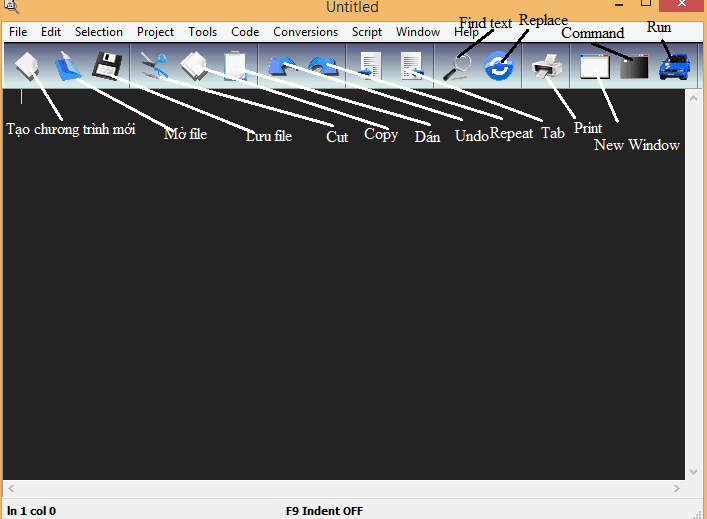
\includegraphics[scale=0.5]{MASMGiaoDien.png}
				\end{center}
				\caption{Giao diện công cụ MASM32}	
					\label{fig:MASM}		
			\end{figure}
		\end{center}			
	
	
	Trên thanh status bar có các chức năng: Tạo chương trình mới, mở file, lưu file, cut, copy, dán, undo, repeat, tab, find text, replace, print, command, new window, run.\\

	Trước khi biên dịch chương trình cần phải lưu chương trình trước, và trong quá trình làm việc nếu có thay đổi phải lưu trước khi biên dịch vì MASM32 không có cơ chế tự lưu những thay đổi như VC hay VB, và một điều nữa cần chú ý là chức năng Undo trong Masm chỉ cho phép undo 1 hành động vì vậy khi có nhiều thay đổi mà người dùng nghĩ có thể phải undo thì nên save trước , nếu cần phục hồi lại thì exit và không save thì nó sẽ ở trạng thái ở lần save cuối cùng. Ví dụ nếu đã có mã code và bây giờ cần biên dịch vào Menu item: Project, trong menu Project có các mục sau: 
		\begin{itemize}
			\item[•] Compile Resource File: biên dịch file resource, file resource có phần mở rông *.rc file này chứa các tàì nguyên như Icon, DialogBox, Bitmap... mà chương trình sử dụng. 
		\item[•] Assemble Asm file: Tạo file *.Obj từ file .asm. 
		\item[•]  Link Obj: từ file Obj link tới các tài nguyên cần thiết để tạo file exe.
		 \item[•]  Assemble \& Link: thực hiện cả hai bước trên , việc này sẽ tạo sự thuận tiện cho người lập trình, không phải tốn công thực hiện qua hai bước mới tạo nên file .exe
		 \item[•]  Build all: Chức năng này có tác dụng biên dịch cả file resource, và tạo file .exe. Chức năng này được sử dụng khi  có thay đổi những tài nguyên ở file resource. Còn nếu chỉ thay đổi về code trong chương trình thì nên sử dụng Assemble \& link, nó sẽ rút ngắn thời gian biên dịch.
		 \item[•]  Run Makeit.bat: nếu muốn có một file Makeit.bat và muốn sử dụng nó để biên dịch thay vì xài những tùy chọn biên dịch mặc định của MASM. Cũng với những chức năng trên nhưng có thêm console thì khi chạy chương trình ccòn kèm theo một cửa sổ dòng lệnh.
		   \item[•]  Run Program: để chạy thử chương trình sau khi biên dịch. 
		\end{itemize}
		

